\subsection{Nao Hardware}
The Nao Humanoid Platform is made by Aldebaran Robotics. 
Figure~\ref{fig:crrl_nao_coronal1} shows a picture of the Nao at the
Control/Robotics Research Lab of NYU Polytechnic School of Engineering.
The robot weighs $5.4 kg$ and has a maximum forward velocity over flat
terrain of approximately $1 \frac{m}{s}$.
It has 25 degrees-of-freedom (DoF) embodied via a 2 DoF head, two 5 DoF legs,
two 5 DoF arms, two 1 DoF hands, and a 1 DoF hip.
Figure~\ref{fig:nao_joints1} shows a diagram locating each of the joints on
the robot.
% Sonars, joint sensors, cameras, foot sensors, IMU, bumpers and buttons.
Each joint has an absolute angular position encoder, while the feet each have
four force sensitive resistors to detect ground contact.
The head has two color cameras, one that faces forward and the other that faces
downward to get a view of the terrain. The chest contains a 2-axis gyroscope and
a 3-axis accelerometer for inertial measurement, and two sonar transmitter-receiver
pairs for measuring the range to obstacles.
Figure~\ref{fig:nao_features1} shows a diagram locating the various robot sensors,
including those not listed above.
% Battery life, weight, top speed (before and after Lidar), sonar ranges, camera angles and pixels,
The sonars have a minimum range of $0.25 m$ and a maximum range of $2.55 m$.
They have a resolution of $1 cm$ and detect any obstacle within a $60^\circ$
cone. The cameras have a $1.22 Mp$ resolution, $30 Hz$ frame rate,
a horizontal field-of-view of $60.9^\circ$, and a vertical field-of-view of
$47.6^\circ$.
% CPU type and speed, RAM, storage space, USB, Ethernet, WiFi.
The robot is equipped with a 1.6 GHz Intel\textsuperscript{\textregistered}
Atom\textsuperscript{TM} CPU, 1 GB of RAM, and 2 GB of Flash memory.
It also has Gigabit Ethernet, 802.11 b/g/n WiFi, and USB 2.0. 
Nao's operating system is called NAOqi OS which is a customized version of
Gentoo Linux. Being a Linux distribution, the robot can be easily accessed
using ssh, scp, and ftp. This allows familiar command line tools to be used
to script behavior and manage services.
The robot can be natively programmed using the provided C++ or Python API.

% Ok, now briefly review what's to come in the subsubsections.
The Nao is a very feature rich platform suitable for a variety of autonomous
applications. The following sections will review specific aspects of the robot
relevant to Chapters~\ref{ch:results_navigation} and~\ref{ch:results_crawling}.


\begin{figure}
\centering
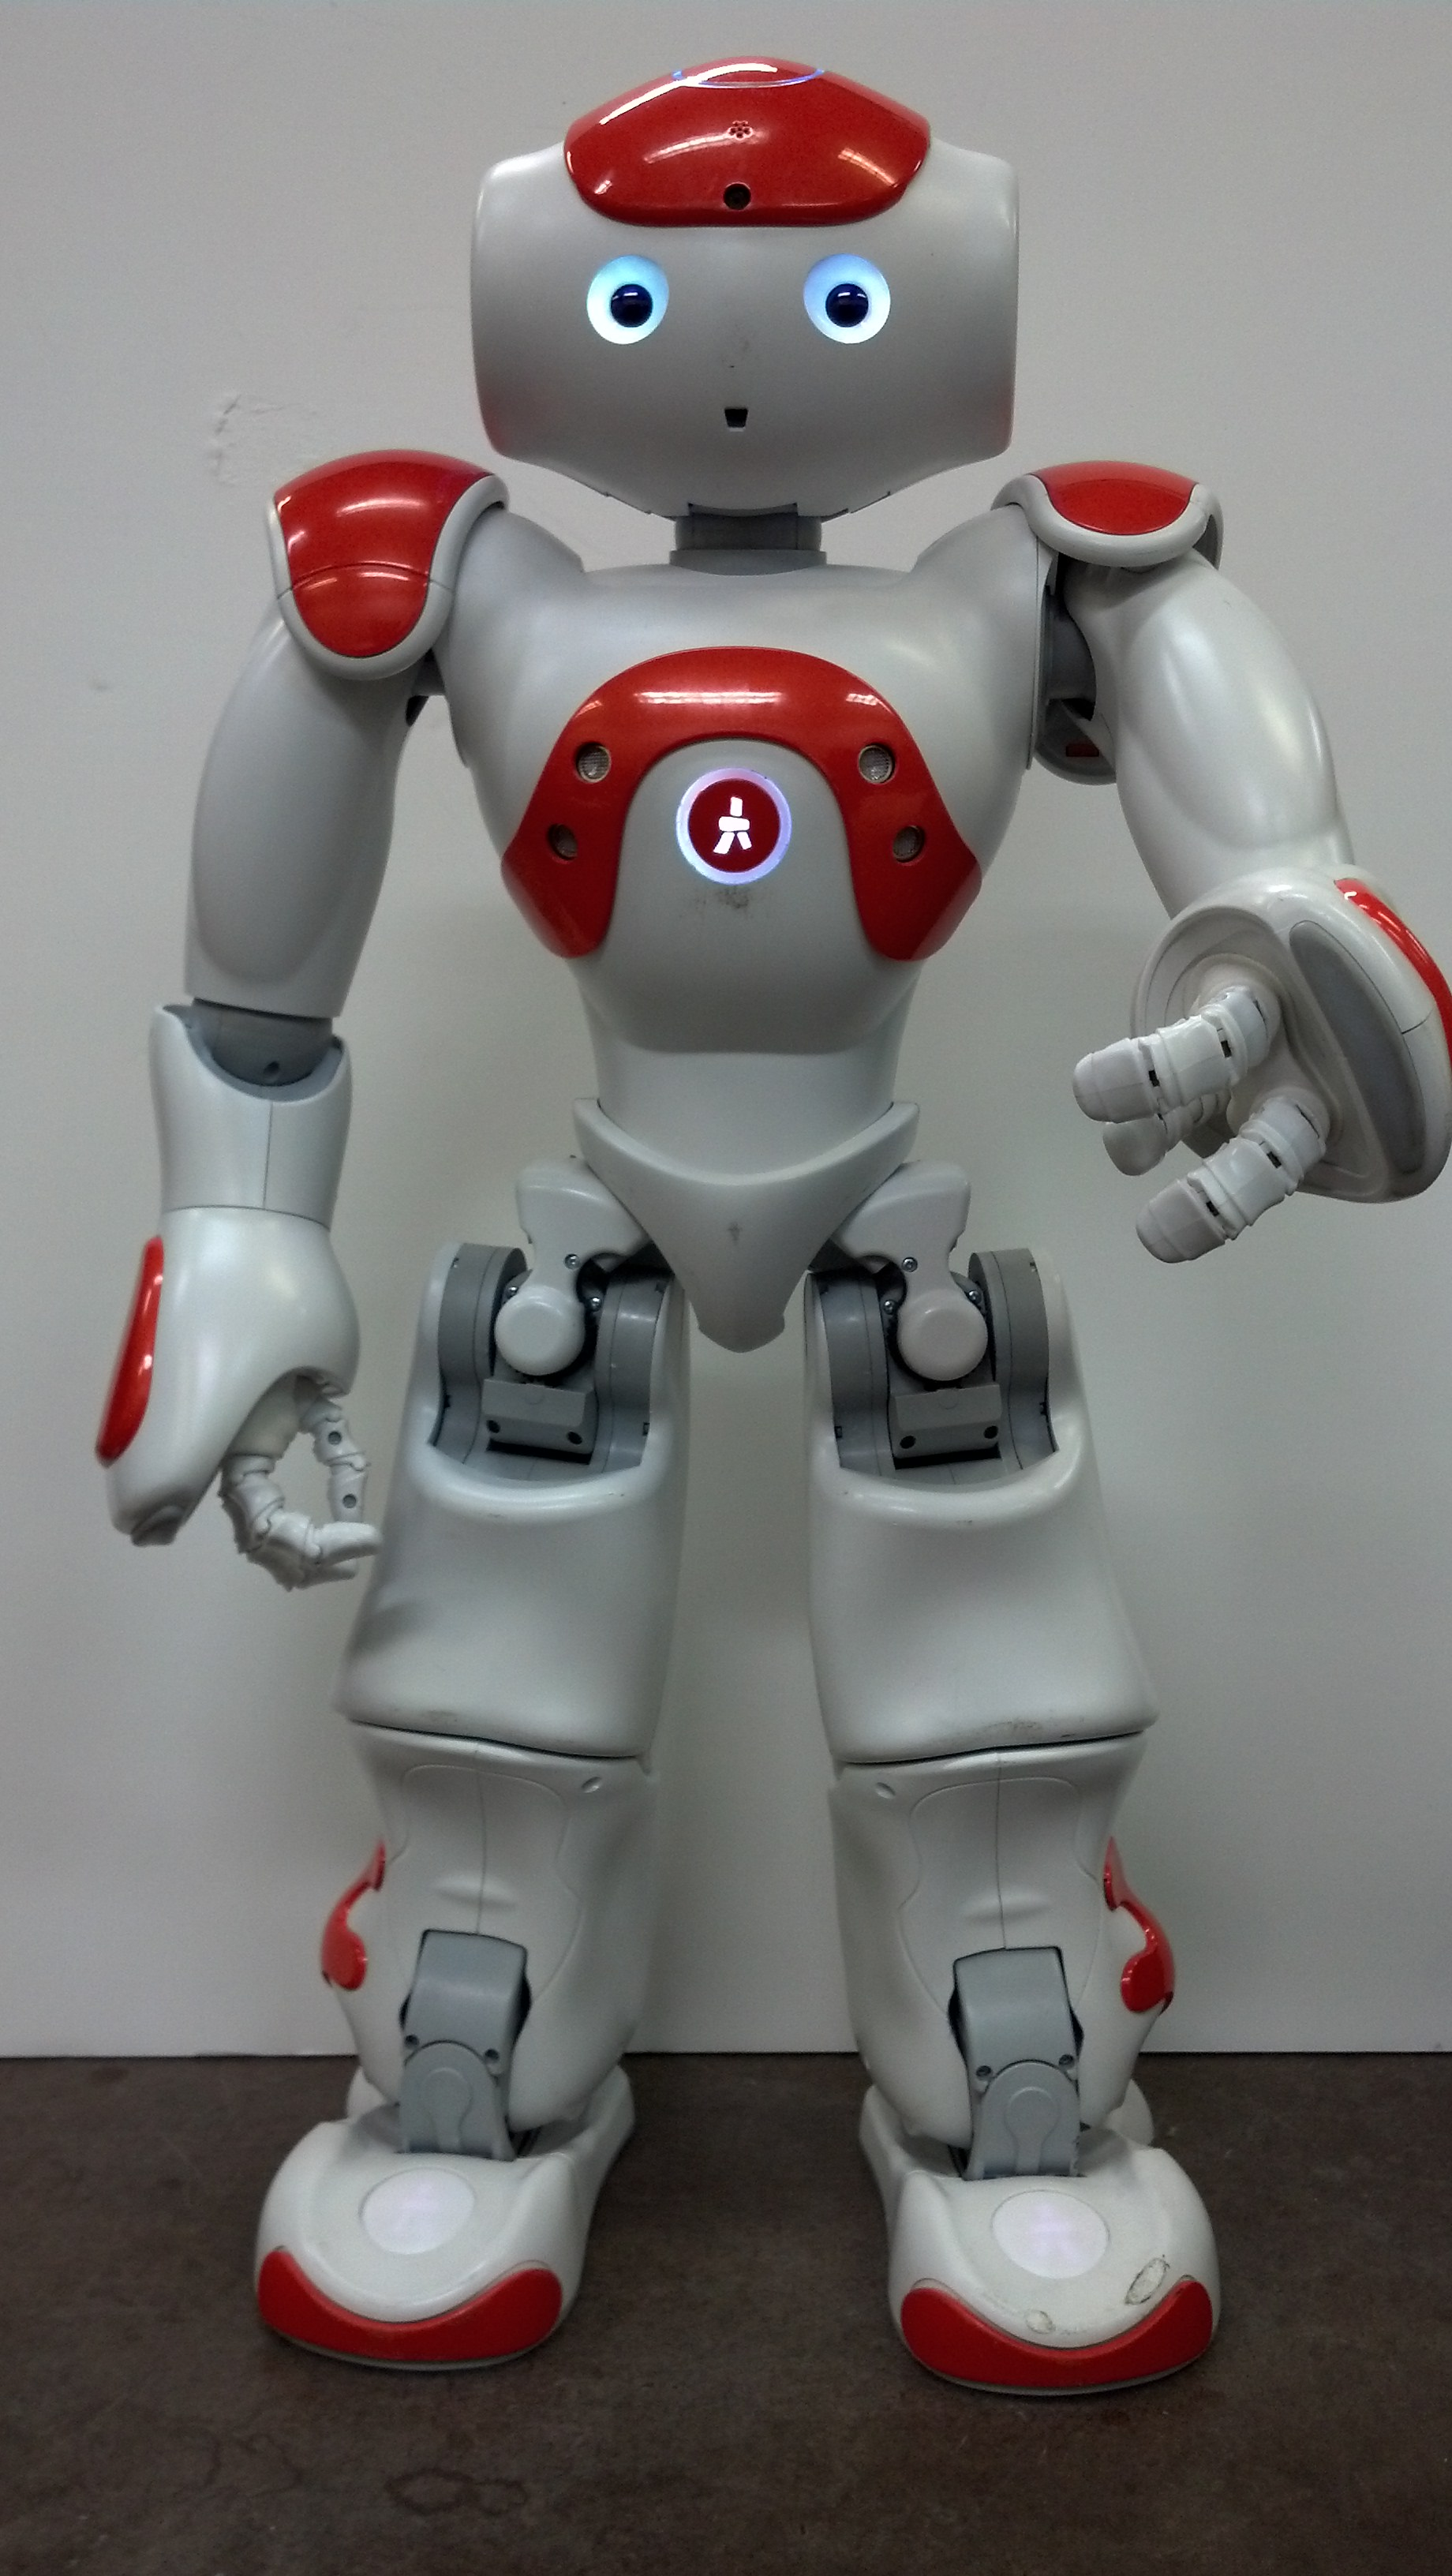
\includegraphics[height=0.4\textheight]{nao_coronal1.jpg}
\caption{Figure showing the Nao Humanoid Platform at the Control/Robotics
         Research Lab at NYU Polytechnic School of Engineering.}
\label{fig:crrl_nao_coronal1}
\end{figure}

\begin{figure}
\centering
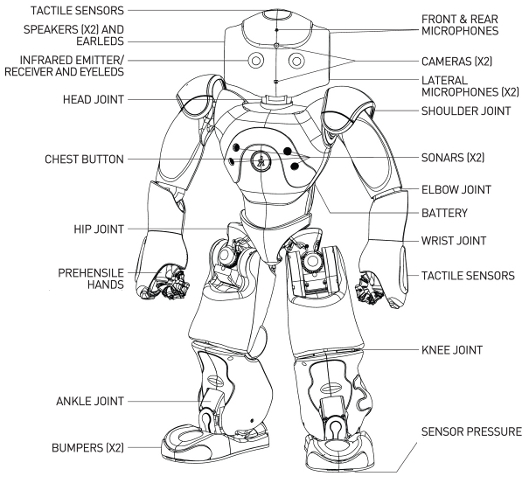
\includegraphics[width=0.4\textheight]{nao_diagrams/nao_h25_pres.png}
\caption{Figure locating the various features on the robot.}
\label{fig:nao_features1}
\end{figure}

\begin{figure}
\centering
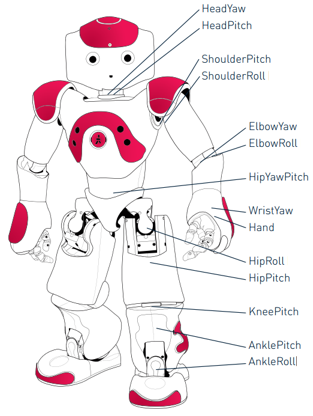
\includegraphics[height=0.4\textheight]{nao_diagrams/hardware_motortype_h25V5.png}
\caption{Figure indicating the various joint locations and their names.}
\label{fig:nao_joints1}
\end{figure}

\FloatBarrier

\subsubsection{Frame Definitions}
The NAOqi API defines three frames that can be seen in Figure~\ref{fig:nao_frames1}.
They are \textbf{FRAME_TORSO}, \textbf{FRAME_ROBOT}, and \textbf{FRAME_WORLD}.
The first two frames, \textbf{FRAME_TORSO} and \textbf{FRAME_ROBOT}, are rigidly
attached to the robot, while \textbf{FRAME_WORLD} is an inertial frame initialized
when the robot first starts.



\begin{figure}
\centering
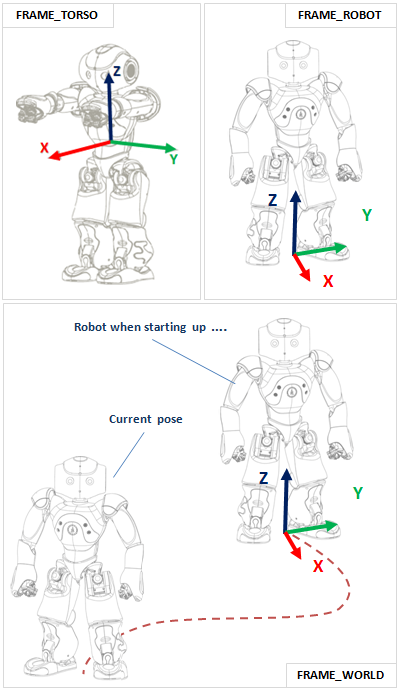
\includegraphics[height=0.75\textheight]{nao_diagrams/frame_definition_combo.png}
\caption{Nao frames.}
\label{fig:nao_frames1}
\end{figure}

\begin{figure}
\centerline{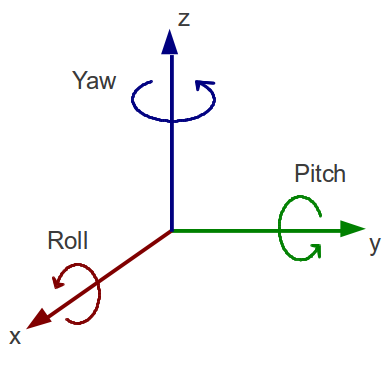
\includegraphics[width=0.5\textwidth]{nao_diagrams/rollPitchYaw.png}
}
\caption{Definition of roll pitch and yaw.}
\label{fig:nao_rpy_def1}
\end{figure}

\subsubsection{Kinematics or Link Joints things}
Talking about what the links are, where, symmetry.

\begin{figure}
\centerline{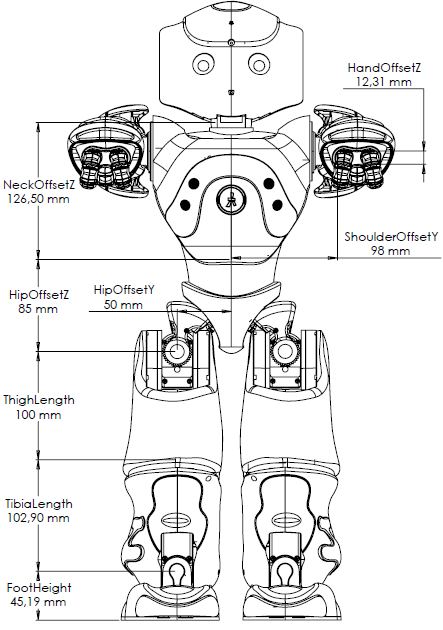
\includegraphics[width=0.45\textwidth]{nao_diagrams/hardware_lengthfront_3.3.png}
            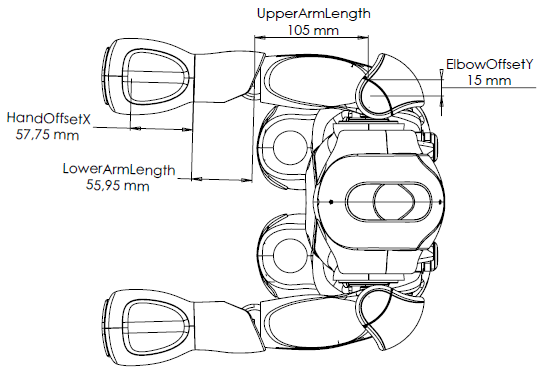
\includegraphics[width=0.55\textwidth]{nao_diagrams/hardware_lengthup_3.3.png}
}
\caption{Nao link lengths.}
\label{fig:nao_link_lengths1}
\end{figure}

\begin{figure}
\centering
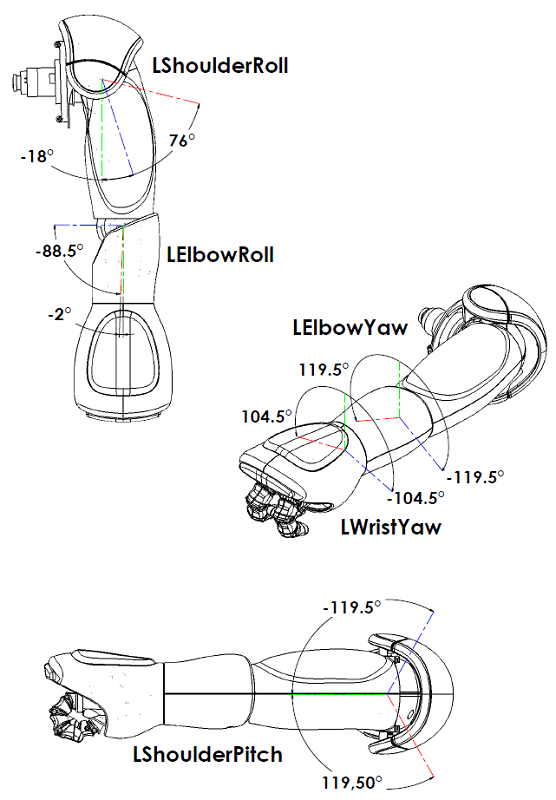
\includegraphics[width=\textwidth]{nao_diagrams/hardware_larmjoint_3.3.png}
\caption{Figure showing left arm}
\label{fig:nao_arm_joints_left1}
\end{figure}

\begin{figure}
\centering
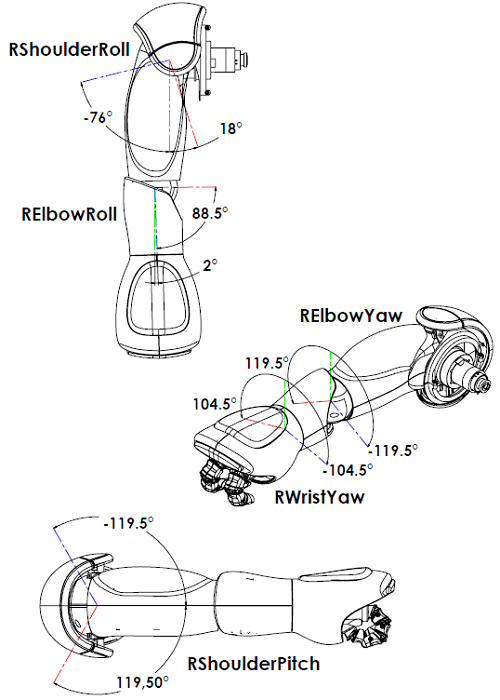
\includegraphics[width=\textwidth]{nao_diagrams/hardware_rarmjoint_3.3.png}
\caption{Figure showing right arm}
\label{fig:nao_arm_joints_right1}
\end{figure}

\begin{figure}
\centering
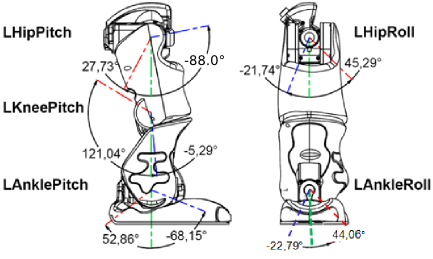
\includegraphics[width=\textwidth]{nao_diagrams/hardware_llegjoint.png}
\caption{Figure showing left leg}
\label{fig:nao_leg_joints_left1}
\end{figure}

\begin{figure}
\centering
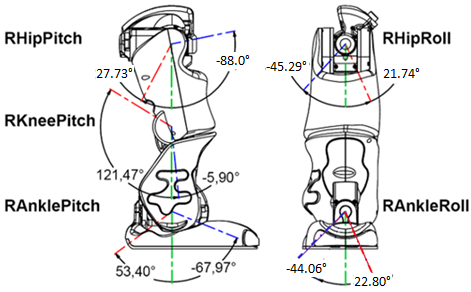
\includegraphics[width=\textwidth]{nao_diagrams/hardware_rlegjoint.png}
\caption{Figure showing right leg}
\label{fig:nao_leg_joints_right1}
\end{figure}

\begin{figure}
\centering
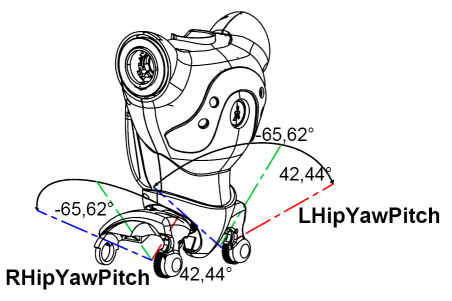
\includegraphics[width=\textwidth]{nao_diagrams/hardware_pelvisjoint.png}
\caption{Figure showing hip yaw-pitch}
\label{fig:nao_hip_yawpitch1}
\end{figure}


Need diagram showing arm symmetry for crawl results. 
\begin{figure}
\centering
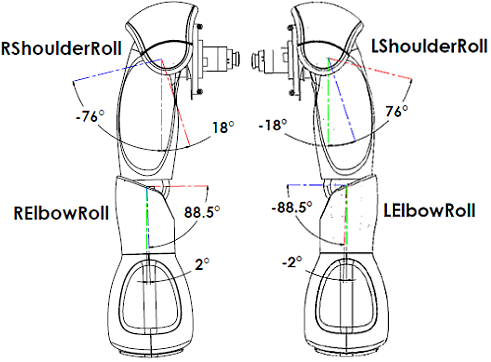
\includegraphics[width=\textwidth]{hardware_r_and_l_armjoint.png}
\caption{Figure showing arm joints and how they are a reflection.}
\label{fig:nao_arm_joints_reflect1}
\end{figure}

\subsubsection{Joint Torques}
% Motor torques. (Important for Chapter~\ref{ch:crawl_gait})
Talking about the joint motor torques, tables, gearboxes, blah.

\subsubsection{Postures}
Talking about the different postures of the robot.

\begin{figure}
\centerline{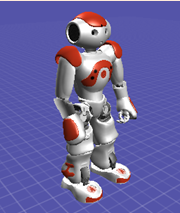
\includegraphics[width=0.33\textwidth]{posture/posture_stand.png}
            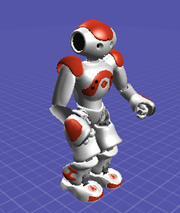
\includegraphics[width=0.33\textwidth]{posture/posture_standinit.png}
            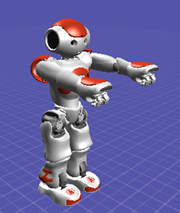
\includegraphics[width=0.33\textwidth]{posture/posture_standzero.png}
}
\vspace*{0.05in}
\centerline{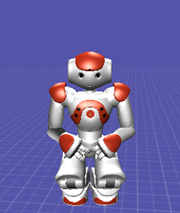
\includegraphics[width=0.33\textwidth]{posture/posture_crouch.png}
            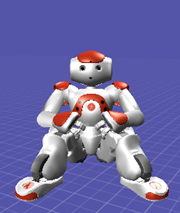
\includegraphics[width=0.33\textwidth]{posture/posture_sit.png}
            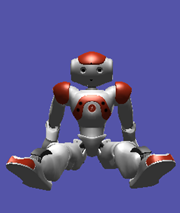
\includegraphics[width=0.33\textwidth]{posture/posture_sitrelax.png}
}
\vspace*{0.05in}
\centerline{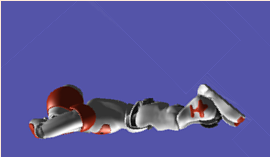
\includegraphics[width=0.5\textwidth]{posture/posture_lyingbelly.png}
            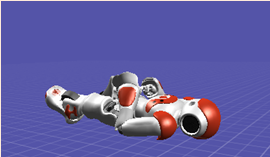
\includegraphics[width=0.5\textwidth]{posture/posture_lyingback.png}
}
\caption{Figure showing postures.}
\label{fig:nao_postures1}
\end{figure}
